\documentclass[tikz,border=2pt]{standalone}
\usepackage{tikz}
\usetikzlibrary{positioning}
\begin{document}
% Namikawa--Ueno type: II^*-I^*_l-t
% Target MRNC type: II^*-I^*_l-t
% Adapted from Tim Dokchitser picture: I^*_{{\it n}}\e({\it m})II^*
% Parameter substitution: n -> l, m -> t
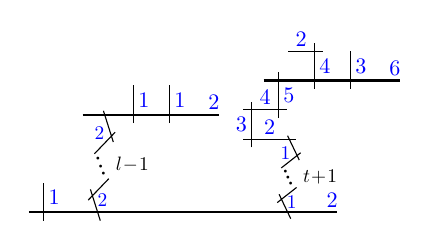
\begin{tikzpicture}[xscale=0.57,yscale=0.62]
\draw[thick,shorten >=2] (-1/3,0)--(20/3,0) node[inner sep=2pt,blue,above left,scale=0.8] {2};
\draw[shorten <=-3pt] (0,0)--node[inner sep=2pt,scale=0.8,blue,right] {1} (0,3/5);
\draw (6/5,0) 
    ++(0.06,-0.17)--++(-0.22,0.64)++(0.11,-0.24)  
    ++(0,0.02)
      node[blue,scale=0.7,inner sep=1,anchor=west]{2}
    ++(0,-0.02)
    ++(-0.16,0.02)--++(0.46,0.44)++(-0.12,0.08)  
    node{$\cdot$} ++(-0.06,0.16) node{$\cdot$}
    ++(-0.06,0.16) node{$\cdot$}++(0.17,-0.12)    node[auto,inner sep=5,scale=0.7,anchor=west]{$l\!-\!1$}
    ++(-0.25,0.23)--++(0.46,0.44)++(-0.19,0.04)   
    ++(0,-0.05)
      node[blue,scale=0.7,inner sep=1,anchor=east]{2}
    ++(0,0.05)
    ++(0.19,-0.04)++(-0.04,-0.2)--++(-0.22,0.64);
\draw[thick,shorten >=2] (13/15,2)--(121/30,2) node[inner sep=2pt,blue,above left,scale=0.8] {2};
\draw[shorten <=-3pt] (2,2)--node[inner sep=2pt,scale=0.8,blue,right] {1} (2,13/5);
\draw[shorten <=-3pt] (14/5,2)--node[inner sep=2pt,scale=0.8,blue,right] {1} (14/5,13/5);
\draw (163/30,0) 
    ++(0.07,-0.13)--++(-0.26,0.5)++(0.12,-0.19)  
    ++(0,0.02)
      node[blue,scale=0.7,inner sep=1,anchor=west]{1}
    ++(0,-0.02)
    ++(-0.16,0.02)--++(0.43,0.31)++(-0.13,0.07)  
    node{$\cdot$} ++(-0.06,0.12) node{$\cdot$}
    ++(-0.06,0.12) node{$\cdot$}++(0.17,-0.1)    node[auto,inner sep=5,scale=0.7,anchor=west]{$t\!+\!1$}
    ++(-0.26,0.19)--++(0.43,0.31)++(-0.18,0.04)   
    ++(0,-0.04)
      node[blue,scale=0.7,inner sep=1,anchor=east]{1}
    ++(0,0.04)
    ++(0.18,-0.04)++(-0.03,-0.15)--++(-0.26,0.5);
\draw[shorten <=-3pt, shorten >=-3pt] (163/30,3/2)--node[inner sep=2pt,scale=0.8,blue,above] {2} (139/30,3/2);
\draw[shorten <=-3pt, shorten >=-3pt] (139/30,3/2)--node[inner sep=2pt,scale=0.8,blue,left] {3} (139/30,21/10);
\draw[shorten <=-3pt, shorten >=-3pt] (139/30,21/10)--node[inner sep=2pt,scale=0.8,blue,above] {4} (157/30,21/10);
\draw[shorten <=-3pt, shorten >=-3pt] (157/30,21/10)--node[inner sep=2pt,scale=0.8,blue,right] {5} (157/30,27/10);
\draw[thick,shorten >=2] (49/10,27/10)--(121/15,27/10) node[inner sep=2pt,blue,above left,scale=0.8] {6};
\draw[shorten <=-3pt, shorten >=-3pt] (181/30,27/10)--node[inner sep=2pt,scale=0.8,blue,right] {4} (181/30,33/10);
\draw[shorten <=-3pt] (181/30,33/10)--node[inner sep=2pt,scale=0.8,blue,above] {2} (163/30,33/10);
\draw[shorten <=-3pt] (41/6,27/10)--node[inner sep=2pt,scale=0.8,blue,right] {3} (41/6,33/10);
\end{tikzpicture}
\end{document}
